\subsection{Problems}

%%%%%%%%%%%%%%%%%%%%%%%%%%%%%%%%%%%%%%%%%%%%%%%%%%%%

\noindent {\bf Problem \thesection.\theprob}\stepcounter{prob}

The performance curve of a pump is $H_p = 70-10000\,Q^2$. This pump is connected to two pipe systems with characteristic curves $H_{s1} = 5000\,Q^2+10$ and $7500\,Q^2+15$. In these formulae, the head is in meters, and the unit of the volumetric flow rate is $\frac{\mathrm{m^3}}{\mathrm{s}}$. Find the operation point, if the two pipe systems are connected (a) in series, or (b) in parallel to the pump. Draw the performance curves in both cases!

Solution: when the pipe systems are in series connection, the volumetric flow rate through them is the same, and in the calculation of the performance curves, the heads are summed at each volumetric flow rate. This means:
\begin{equation*}
H_{s,ser} = H_{s1} + H_{s2} = 12500\,Q^2+25.
\end{equation*}
In the operation point, the head of the pump equals the head required by the system:

\begin{align*}
& H_{s,ser} = H_p, \\
& 12500\,Q^2+25=70-10000\,Q^2,\\
& Q_{ps} = \sqrt{\frac{45}{22500}} = 0.04472~\frac{\mathrm{m^3}}{\mathrm{s}}, \\
& H = H_p(Q_{ps}) = H_{s,ser} = 70 - 10000\cdot 0.04472^2 = 50~\mathrm{m}.
\end{align*}

When the two pipe systems are connected in parallel, the pressure drop/head is the same on them, while their volumetric flow rates are different. In this case, to calculate the characteristic curve of the total system, the volumetric flow rates should be summed at each head. To do this,  we need to rearrange the performance curves to be functions of the head:
\begin{align*}
& H_p = 70-10000\,Q^2 \rightarrow Q_p = \frac{\sqrt{70-H}}{100} \\
& H_{s1} = 5000\,Q^2+10 \rightarrow Q_{s1} = \frac{\sqrt{2}\,\sqrt{H-10}}{100} \\
& H_{s2} = 7500\,Q^2+15 \rightarrow Q_{s2} = \frac{\sqrt{3}\,\sqrt{H-15}}{150} .
\end{align*}
Note that the expressions above are only valid for a certain $H$ interval, since the argument of the square root function cannot be negative. Calculating the sum of the two parallel pipes, then equating the pump and the system, solving for $H$, the operating point can be identified:
\begin{align*}
& Q_{s,par} = Q_{s1} + Q_{s2} = \frac{\sqrt{2}\,\sqrt{H-10}}{100}+\frac{\sqrt{3}\,\sqrt{H-15}}{150}  = Q_p = \frac{\sqrt{70-H}}{100}\\
& H =  20.03~\mathrm{m}, \\
& Q = 0.07069~\frac{\mathrm{m^3}}{\mathrm{s}}.
\end{align*}

The performance curves are displayed in Figure \ref{fig_example1}.

\begin{figure}[!htb]
\centering
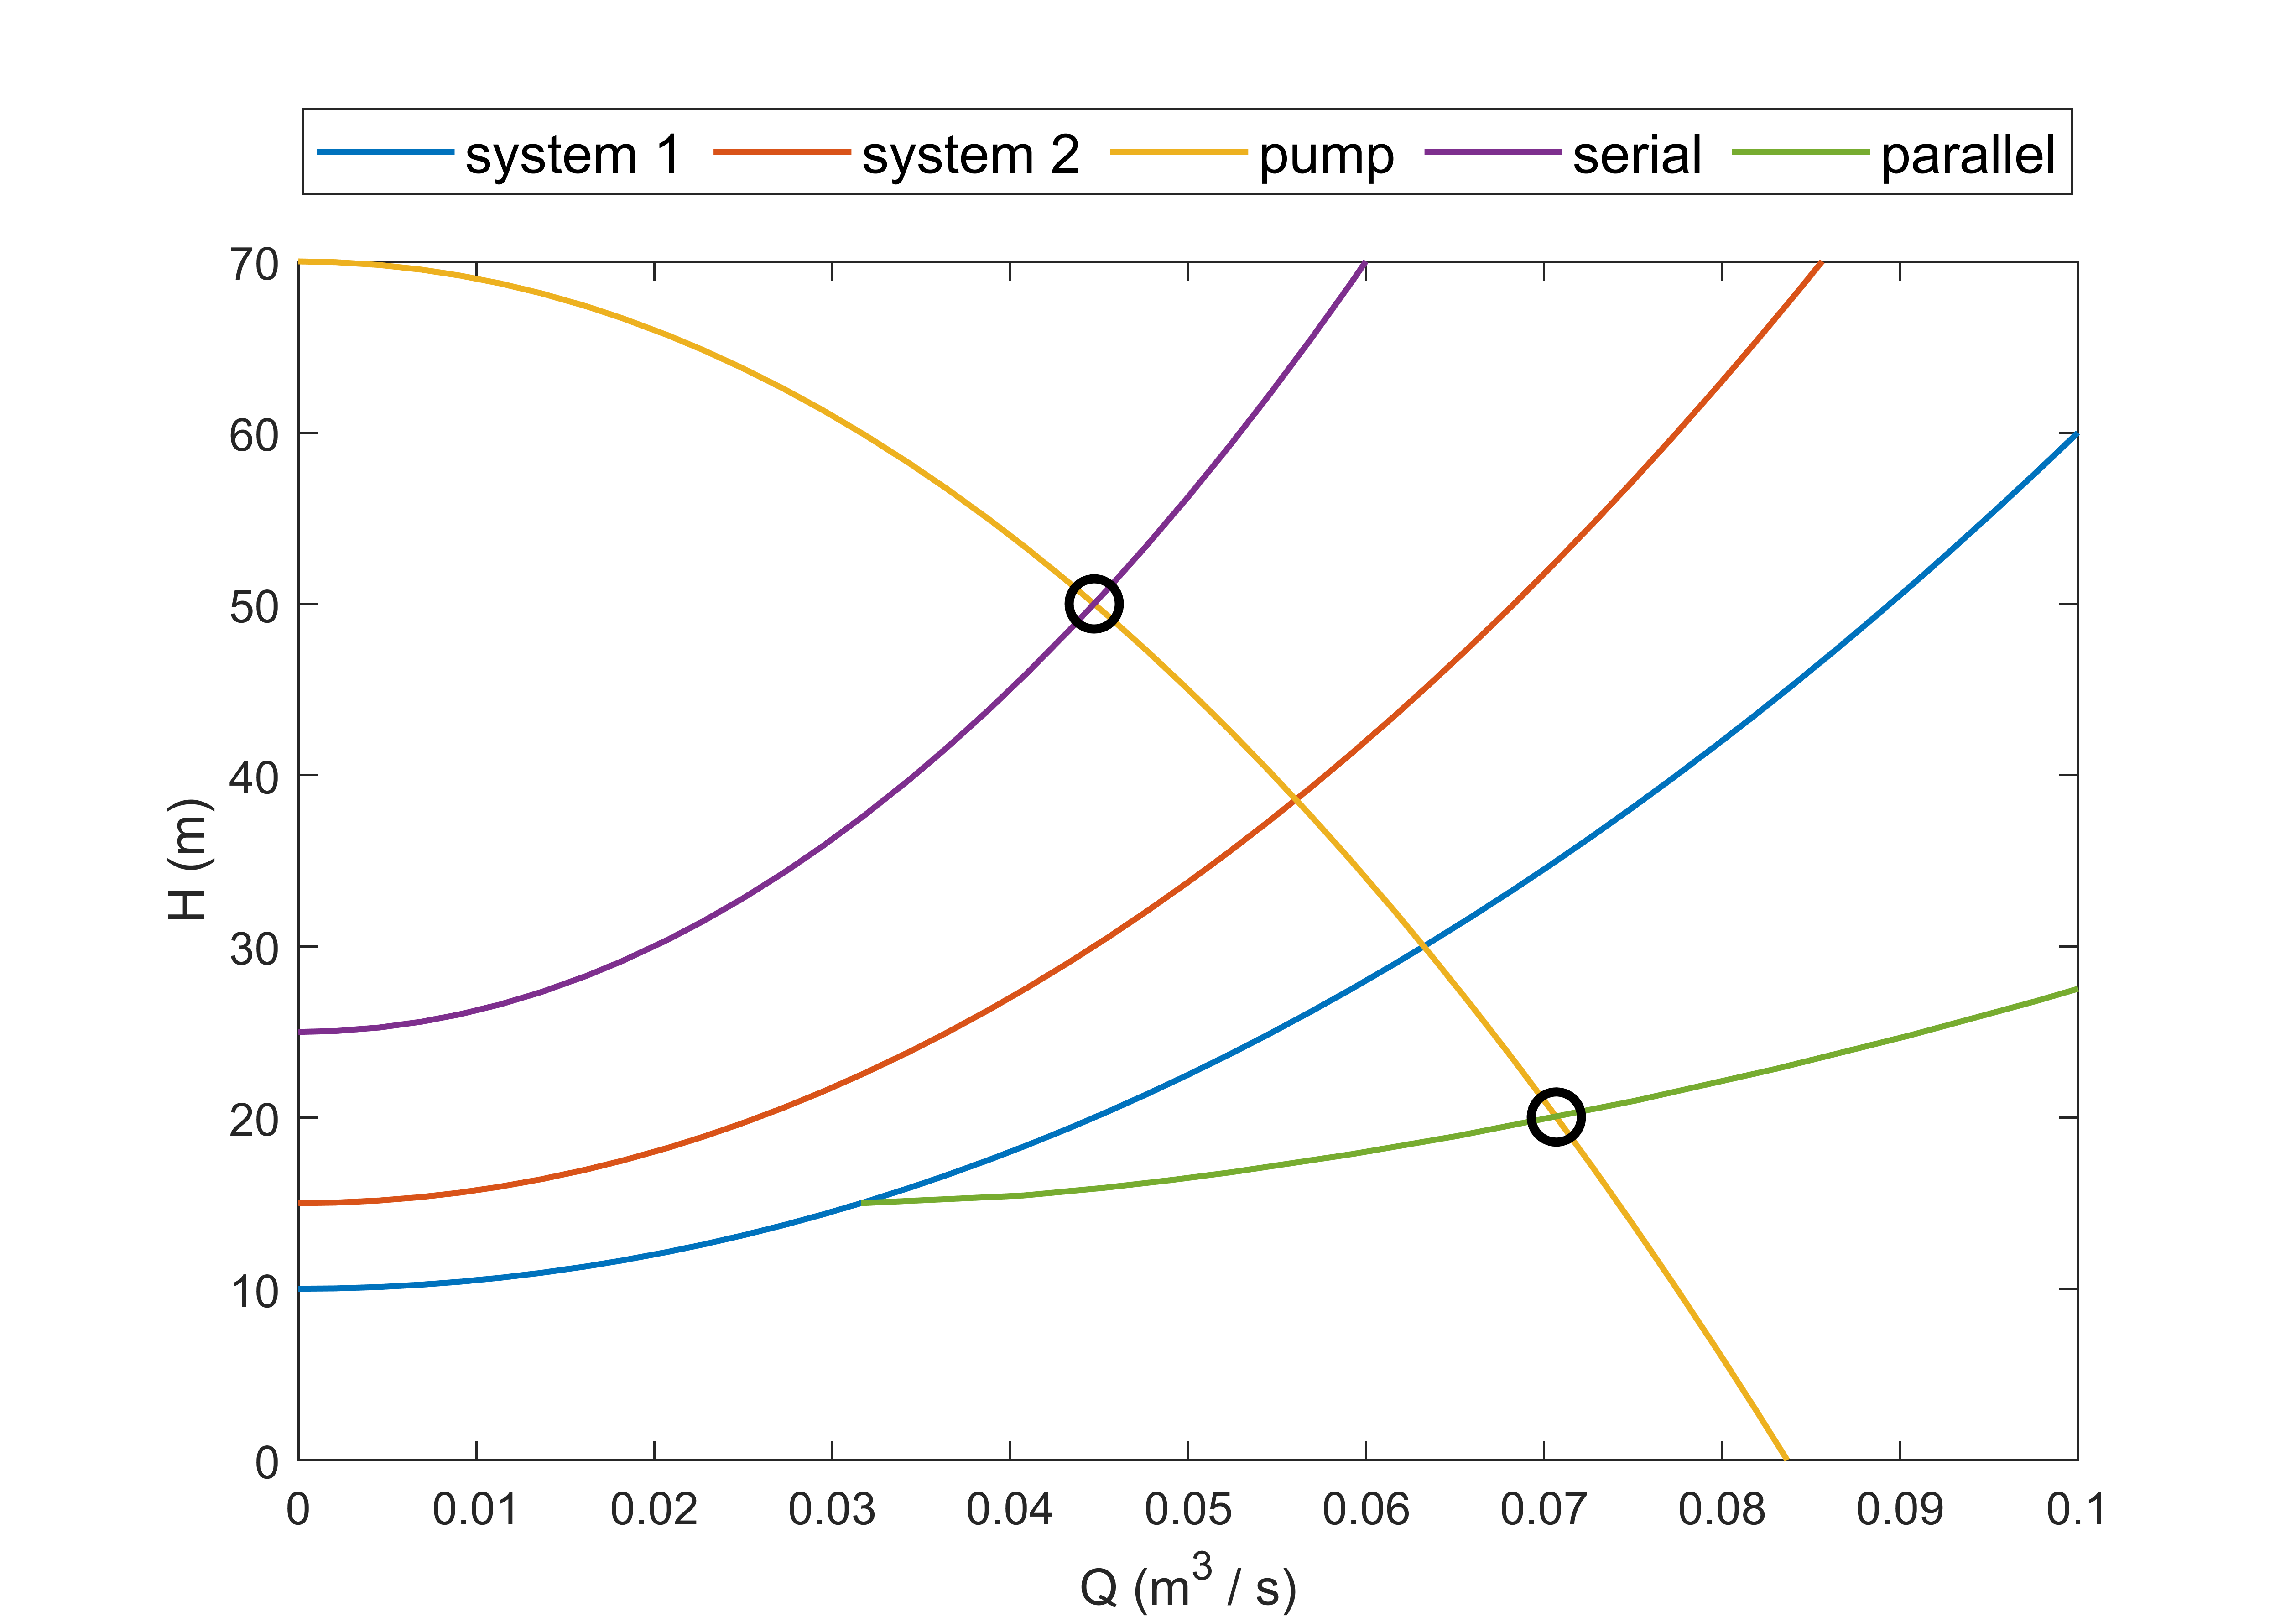
\includegraphics[width=0.8\textwidth]{figs/problem_5_par_1.png} 
\caption{ Performance curves of the problem. The circles denote the operation points.}
\label{fig_example1}
\end{figure}

%%%%%%%%%%%%%%%%%%%%%%%%%%%%%%%%%%%%%%%%%%%%%%%%%%%%

\vspace{1cm}
\noindent {\bf Problem \thesection.\theprob}\stepcounter{prob}

Two pumps, with performance curves $H_{p1} = 50 - 30000\cdot Q^2$ and $H_{p2} =  40 - 20000\cdot Q^2$ are conveying water through a pipe system that's characteristic curve is $H_s = 3 + 7250\cdot Q^2$. Find the operating points if the two pump are connected (a) in series or (b) in parallel! (Solution: $H_{ser} = 14.02~\mathrm{m}$, $Q_{ser} = 0.03898~\frac{\mathrm{m^3}}{\mathrm{s}}$, $H_{par} = 25.43~\mathrm{m}$, $Q_{par} = 0.05562~\frac{\mathrm{m^3}}{\mathrm{s}}$)

%%%%%%%%%%%%%%%%%%%%%%%%%%%%%%%%%%%%%%%%%%%%%%%%%%%%
%peldatar 6.1

\vspace{1cm}
\noindent {\bf Problem \thesection.\theprob}\stepcounter{prob}

A pump that's performance curve is $H_I (\mathrm{m}) = 70 - 50000 \frac{\mathrm{s^2}}{\mathrm{m^5}} Q^2$, conveys water through a pipe system with characteristic curve $H_s (\mathrm{m}) = 20 + 10000 \frac{\mathrm{s^2}}{\mathrm{m^5}} Q^2$. Find the volumetric flow rate! The volumetric flow rate is increased to $Q=0.032~\frac{\mathrm{m^3}}{\mathrm{s}}$, using a second pump with performance curve $H_{II} (\mathrm{m}) = 80 - 50000 \frac{\mathrm{s^2}}{\mathrm{m^5}} Q^3$. The operating point of the system is set by a throttle valve at the pressure side. How would the loss power be smaller: if the two pumps were connected in series or in parallel? (Solution: $Q=0.0285~\frac{\mathrm{m^3}}{\mathrm{s}}$, $P_{ser}' = 5.45~\mathrm{kW}$, $P_{par}' = 9.88~\mathrm{kW}$)

%%%%%%%%%%%%%%%%%%%%%%%%%%%%%%%%%%%%%%%%%%%%%%%%%%%%

\vspace{1cm}
\noindent {\bf Problem \thesection.\theprob}\stepcounter{prob}

Two pump operate in parallel. The performance curve of the first pump and it's pressure side pipeline is the following: $H_{pI} = 40 - 0.17Q^2$, $H_{s,I} = 5 + 0.4Q ^2$; the data for the second pipe is $H_{pII} = 27 - 0.135Q^2$, $H_{s,II} = 0.8Q ^2$. The head in in meters, and the unit of the volumetric flow rate is $\frac{\mathrm{m^3}}{h}$. These two pipes are joined, and convey water through a third pipeline with characteristic curve $H_{s,III} = -3 + 0.63Q ^2$. Find the operating point! (Solution: $Q = 6.473~\frac{\mathrm{m^3}}{h}$, $H=23.4~\mathrm{m}$.)